% English review draft. XeLaTeX -> BibTeX -> XeLaTeX twice.
% Technical evidence and a prospective study, not participant-study results.
\RequirePackage[T1]{fontenc}
\documentclass[conference,10pt,letterpaper]{IEEEtran}
\usepackage{fontspec}
\setmainfont{TeX Gyre Termes}
\setsansfont{TeX Gyre Heros}
\setmonofont{Latin Modern Mono}
\usepackage{amsmath,amssymb,graphicx,booktabs,tabularx,array,balance,cite}
\usepackage[hidelinks]{hyperref}
\usepackage{url}
\newcolumntype{Y}{>{\raggedright\arraybackslash}X}
\graphicspath{{figures/}}
\newcommand{\sys}{CoVisStudio}
\hyphenation{CoVisStudio}
\title{CoVisStudio: Separating Evidence from Edit Scope\\in Full-Duplex Collaborative Visual Analysis}
\author{\IEEEauthorblockN{Anonymous review draft}}
\begin{document}
\maketitle
\begin{abstract}
When people revise analytical dashboards with an AI assistant, reusing previously discussed objects need not mean restoring their historical filters. Full-duplex interaction allows revisions during explanation and execution, while generated speech, delivered speech, and the visible canvas can differ. We present CoVisStudio, which represents a revision through object provenance, current targets and changes, and retained or released conditions. A correctable revision card exposes this interpretation over execution capabilities shared with a strong direct-editing baseline. The system separately records commits, rendering, visibility, and output-sample playback. A local browser workflow passed 24 mechanism checks. Earlier real-model diagnostics exposed unexecuted promises, argument rejection, and outdated follow-up images. After explicit argument-contract and image-order changes, two bounded checks completed reranking and historical-member transfer, with independently verified data, matching image delivery, and natural final playback. Earlier failures remain separate records. We specify a prospective two-condition, full-duplex study of correctness, understanding, and repair cost. The evidence supports implementation feasibility; user benefit remains to be tested.
\end{abstract}
\begin{IEEEkeywords}
human--AI collaboration, full-duplex speech, visual analytics, intent revision, shared evidence
\end{IEEEkeywords}

\section{Introduction}
Creating a dashboard is rarely a single translation of a complete specification. People inspect charts, select comparison objects, change measures, and narrow the scope as their questions develop. With an AI assistant, collaborators must continually establish what they are discussing, what has changed, and what remains valid. This is coordination around a shared analytical artifact, beyond converting language into chart commands.

Consider three charts showing order volume, low-review rate, and delivery time. A user first examines three priority categories in the Brazilian state of RJ, then moves to MG. During the assistant's explanation, the user asks: ``Use those three categories you just discussed for the two service charts; keep the current region and dates.'' Correct execution must recover the historical members, target the specified current views, and retain MG. Restoring the earlier query or selecting MG's current top three may yield numerically correct charts that answer a different question.

Full-duplex speech provides an entry point for timely revision, but does not ensure shared understanding. Generated words may not have played; a committed chart may not have rendered; a reference to an explanation may concern an earlier set rather than the latest one. The final chart and a complete chat transcript alone cannot establish the evidence available when a revision arose.

Prior work supports ambiguity management, speech--canvas collaboration, and intervention during execution~\cite{datatone,cleo,voca}. Neither interruption nor combining speech with images is our contribution. We ask: \emph{In collaboration that permits revision during delivery, can explicitly separating referenced evidence from the current edit scope help collaborators execute and understand changes, and at what interaction cost?} Both planned conditions use full-duplex interaction; we do not compare it with sequential interaction.

We contribute an implemented revision representation separating historical object identity from current filters, measures, and targets, with a correctable shared card. We also connect inputs, execution, and delivery in a verification workflow, report technical successes and preserved failures, and specify a comparison that retains the baseline's exact-member reuse capabilities. User benefit remains the hypothesis this protocol will test.

\section{Related Work}
\subsection{Natural-Language Analysis and Ambiguity}
DataTone exposes ambiguity and partial query constraints, letting users correct interpretations~\cite{datatone}. Our emphasis is a particular revision ambiguity: historical members can remain relevant while their old calculation scope should not return. We separate object provenance from application scope and record relevant delivered speech and visible versions. This is a change of focus, not evidence that a newer speech interface surpasses ambiguity widgets.

Speech-to-Visualization investigates generating visualization queries from spoken questions and database information~\cite{speechvis}. ChartEditBench evaluates grounded, multi-turn editing of existing charts and code~\cite{charteditbench}. These provide direct foundations for speech-driven creation and chart editing. We examine whether historical-evidence reuse preserves the requested objects and current conditions, rather than adding chart types.

\subsection{Speech and Shared-Canvas Collaboration}
CommSketch combines sketching and narration to communicate design intent~\cite{commsketch}. CLEO tracks user actions in a shared design canvas and selectively revises plans during concurrent human--agent work~\cite{cleo}. VoCa studies speech--canvas coordination, feedback, and user control~\cite{voca}. Shared visual work and mid-execution revision therefore have clear precedents.

Analytical dashboards offer independently checkable members, filters, measures, and untouched views. This makes it possible to examine the case where historical objects remain referable without restoring their scope. That setting alone is insufficient novelty: a fair comparison must determine whether explicit support improves revision and understanding.

\subsection{Full-Duplex Execution and Common Ground}
Full-Duplex-Bench-v3 evaluates tool use under realistic disfluency~\cite{fdbv3}; DuplexAgent-RSI addresses coordination of realtime speech with background execution, including delivery of invalidated results~\cite{duplexagent}. We use interruption and commit management as engineering foundations rather than claiming a new coordination algorithm. Grounding requires collaborators to provide and check evidence of understanding~\cite{grounding}. Accordingly, a correct internal member selection and a user's knowledge of that selection are separate outcomes.

\section{Revision Representation and Method}
\subsection{Referenced Evidence and Current State}
A revision episode comprises a user utterance and subsequent clarification, execution, and repair. It need not equal one provider response: a request can generate tools, follow-up speech, and several delivery events. Let $C_i$ denote the current query configuration of view $i$, including region, dates, order status, measure, and membership rule. Historical evidence $e$ contains its source version and member set $M(e)$. We represent a revision as
\begin{equation}
R=(O,T,\Delta,P,L),
\end{equation}
where $O$ is object provenance, $T$ the current target views, $\Delta$ the explicit changes, $P$ retained conditions, and $L$ explicitly released conditions. The interface organizes these into three parts: \emph{object evidence; targets and changes; retained and released conditions}. They derive from expressed requests and available evidence, not evaluator answers.

In the opening example, $M(e)$ supplies the categories, views 2 and 3 are targets, and MG, current dates, delivered status, and each measure are retained. View 1 is unchanged. ``Release those categories and find MG's top three again'' instead removes fixed membership and establishes an explicit ranking. Keeping a fixed set differs from preserving a dynamic ranking rule.

\subsection{Execution Rules and Correctable Support}
The system lists existing historical charts and saved sets, from which the model can select a candidate identifier. Users can also select evidence directly. Both paths share member resolution; historical reuse copies object identity, not the old region, dates, or measure. For target views,
\begin{equation}
C_i'=\operatorname{patch}(C_i,\Delta_i,M(O)),\quad i\in T,
\end{equation}
and $C_i'=C_i$ for $i\notin T$. Reranking requires a measure and count and releases fixed membership. These rules enforce a stated interpretation; they cannot replace understanding an ambiguous utterance.

An explicit request can compute and commit through one flat-argument \texttt{revise\_analysis} call: targets, membership action, candidate identifier, and changed query fields. B0 and B2 share the compiler, candidate tools, and revision structure. B2 exposes a summary and expandable card; B0 retains direct execution feedback. Thus the treatment is a package of \emph{visible, correctable revision support}, not a different binding algorithm or exclusive access to exact members.

Cards do not impose confirmation on every operation. An unresolved choice pauses publication for clarification; a clear request can apply immediately, leaving its card available for inspection and correction through a new request. Such a card may therefore appear after commitment. Generation, viewport exposure, opening, and successful user confirmation are separately recorded. None alone proves agreement or understanding.

\begin{figure*}[t]
\centering
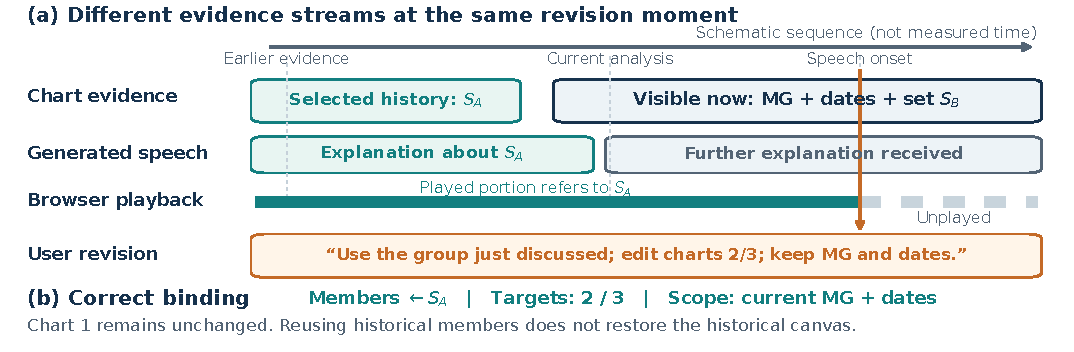
\includegraphics[width=\textwidth]{fig01_revision_timeline.pdf}
\caption{Conceptual full-duplex revision. Historical members remain evidence while the current calculation scope stays in MG. Generated follow-up speech is not necessarily delivered speech. Sequence and set symbols are illustrative, not measured timing or results.}
\label{fig:timeline}
\end{figure*}

\subsection{The Role of Full-Duplex Interaction}
Revision can arrive while an explanation is partially delivered, a tool remains unfinished, or a chart has just changed (Fig.~\ref{fig:timeline}). The challenge includes semantic reference errors even when the selected operation executes correctly, beyond preventing stale results from overwriting newer ones.

On a speech-start event, the system revokes old work's future publication permission and stops old playback before requesting remote cancellation. Earlier lawful commits remain. Guarantees begin with local event handling, not physical speech onset; delivered audio cannot be recalled. An explicitly named RJ set may be resolved without playback position, whereas ``the group you just mentioned'' may depend on delivered explanation. Human coding must establish that dependence. Different candidate sets yielding different charts does not itself show that full-duplex evidence is necessary.

\section{System and Evidence Records}
\subsection{Interface, Data, and Tools}
\sys{} uses an English Vue/ECharts three-chart interface and a FastAPI backend managing sessions, tools, and public chart state. Voice uses Qwen3.8-Omni-Flash-Realtime~\cite{qwenrealtime} and connects only after an explicit start. Charts, conversation, saved sets, historical inspection, and revision cards form the workspace. The card displays actual changed and retained condition values, rather than field names alone.

Queries use real Olist data~\cite{olist}. Order volume, low-review rate, and delivery time retain their implemented definitions. Low-review rate uses valid reviewed orders as the denominator; delivery time uses eligible delivered records. An order can contribute to several category groups, so category counts are not simply summed as a unique-order total.

Tools compute private candidates. Publication jointly checks current request permission and matching chart version. Both conditions share reads, saved-set tools, data computation, and commit rules. Spoken success cannot publish state. Request-scoped receipts distinguish committed, displayed, and no chart changes; an earlier success cannot certify a later request.

\begin{figure*}[t]
\centering
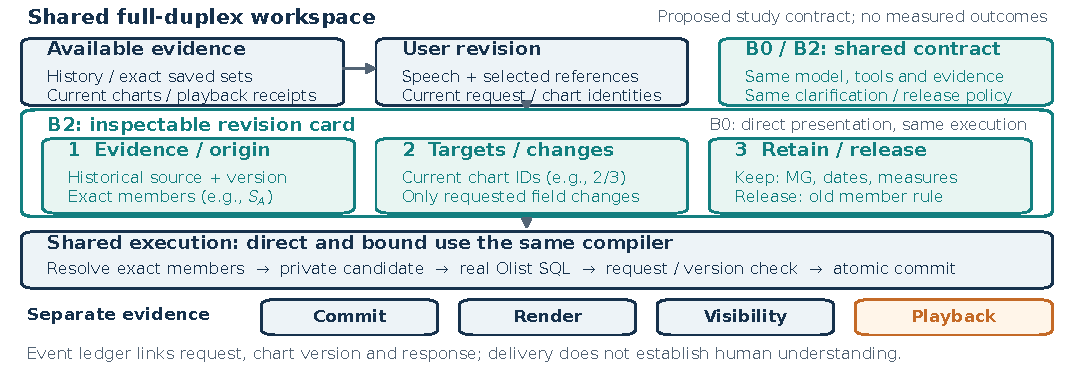
\includegraphics[width=\textwidth]{fig02_revision_architecture.pdf}
\caption{Shared execution and separate verification. B0 and B2 share evidence reads, member resolution, tools, and publication rules; B2 exposes the correctable revision structure. Commit, rendering, visibility, and playback are distinct observations. Application evidence packages do not freeze native provider history.}
\label{fig:architecture}
\end{figure*}

\subsection{Evidence Cutoffs and Actual Delivery}
Request, response, tool, and chart-version identifiers associate events. Browser/server timestamp exchanges estimate clock offset and uncertainty while preserving raw domains. Each application evidence item has a capture time $t_c$, server-availability time $t_a$, provenance, and content digest. At interpretation cutoff $d$, eligibility requires
\begin{equation}
t_c+u\le d\quad\land\quad t_a\le d,
\end{equation}
where $u$ is capture-time uncertainty. An earlier-captured screenshot that has not arrived is not yet available input; indeterminate relationships remain unknown.

AudioWorklet source cursors distinguish received, output, and interrupted unplayed samples, reporting progress about every 1,200 source samples at 24 kHz. A complete received WAV does not prove complete playback, and software output does not establish acoustic listening or word comprehension. Charts separately record publication, completed rendering, and viewport exposure.

Application packages archive versions and digests alongside exact outbound model inputs. Existing content in the native Qwen session is not isolated, so application-level cutoff selection cannot establish a frozen total model context. Aligning words to sample positions remains a separate annotation task.

\section{Preliminary Technical Evaluation}
We report preserved records from November 13, 2026, separating local scripted execution, real-model diagnostics, and a future participant study. Different versions and authored requests are not pooled into an effectiveness estimate.

\subsection{Two Earlier Real-Model Failures}
Two authored Qwen/browser/Olist cases failed despite correct numerical queries (all six final charts matched SQL). Inputs lasted 6.64, 8.56, and 6.32 seconds across segments. One model supplied nested evidence as a JSON string: rejection and the former continuation policy caused 24 failed attempts without a commit. The other committed half-year charts, then promised an overlapping first-quarter change without calling a tool. Playback stopped correctly, but half-year charts remained. Neither plausible speech nor correct arithmetic established requested-goal success.

\subsection{A Local Integrated Workflow}
Flat arguments, single-call revision, failed-receipt termination, and request-scoped outcomes addressed these failures. One scripted local browser/worklet/Olist workflow followed versions $6\rightarrow7\rightarrow8\rightarrow8$: historical-member half-year update, overlapping first-quarter correction retaining MG/members/status/measures and view 1, then an unexecuted promise labeled \emph{No chart changes} (Fig.~\ref{fig:workspace}). All 24 assertions passed across execution, interruption, SQL, untouched views, images, rendering, and closure. They are checks within one workflow, not independent tasks or real-model semantic evidence.

\begin{figure*}[t]
\centering
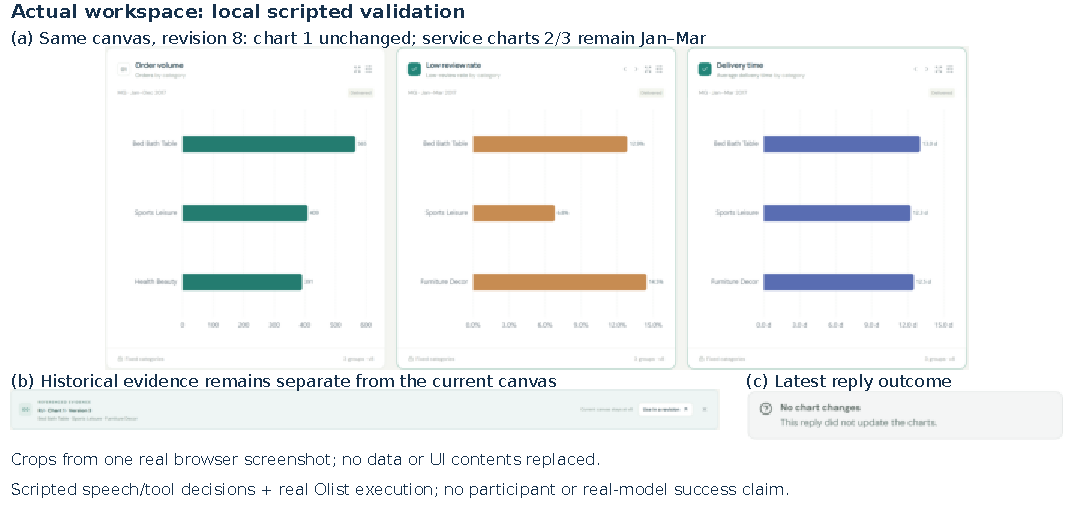
\includegraphics[width=\textwidth]{fig03_actual_workspace.pdf}
\caption{Actual local scripted browser validation, cropped from one screenshot. View 1 retains annual orders, views 2 and 3 show the first quarter, and historical RJ member evidence appears separately. A subsequent second-quarter request receives no tool call, leaving first-quarter charts and a No chart changes receipt. This is neither a real-model success screenshot nor participant evidence.}
\label{fig:workspace}
\end{figure*}

\subsection{An Earlier Eight-Run Real-Model Diagnostic}
Four authored families ran once per runtime path (Table~\ref{tab:matrix}), with complete 4.24--8.56-second clips, connections below 60 seconds, actual playback overlap, and no automatic retries. Preselected historical evidence tested transfer and scope retention, not heard-word reference resolution.

\begin{table}[t]
\caption{Earlier eight-run diagnostic: final analytical outcomes}
\label{tab:matrix}
\centering\small
\begin{tabularx}{\columnwidth}{@{}p{.39\columnwidth}YY@{}}
\toprule
Authored family & Direct path & Bound path \\
\midrule
Historical members, then quarter & Correct; shutdown watchdog & Promise without edit \\
Release fixed set and rerank & Integer-string rejection & Integer-string rejection \\
Historical member transfer & Correct & Cancelled-tool continuation error \\
Keep members, replace measure & Correct & Correct \\
\bottomrule
\end{tabularx}
\end{table}

Four final states met authored goals with commits, rendering, and natural playback; the driver marked three passes. One correct direct run ended playback at 54.634 seconds, crossed its 55-second shutdown watchdog, and closed at 55.752 seconds; it remains failed. Other failures were an unexecuted promise, two integer/string rejections, and cancelled-tool continuation. Some native transcripts were missing from normalized records after epoch advancement. This was not frozen B0/B2 apparatus; a completed finish label did not certify success.

\subsection{Two Subsequent Focused Real-Model Checks}
After transcript-association and native-sequence changes, two authorized checks reused complete cached speech without new TTS or retries. Reranking (02-direct, 19.890 seconds) failed: \texttt{top\_n:"3"} was rejected and revision 6 remained. ASR changed ``Release fixed categories'' to ``These fixed categories.''

Historical transfer (03-bound, 33.750 seconds) committed revision 7, preserving view 1, RJ, third-quarter dates, and target measures, with 14.8 seconds of complete output. All six actual final queries matched independent SQL; the failed reranking goal remained incorrect. Both checks associated late VAD fragments with the continuing request, but did not trigger the specific late-created stale-tool sequence. The transfer still sent a revision-6 follow-up image despite a revision-7 capture. Later repairs do not change this observation.

\subsection{Later Delivery and Contract Checks}
A subsequent bound-path case committed half-year then first-quarter revisions, retaining MG, historical members, measures, and view 1. All 21 archived queries matched independent SQL and both post-commit image sequences matched their revisions. Its original result remains failed: only 28.72/32.08 seconds of final audio played before budget closure (56.109-second connection).

The latest change declares model-facing \texttt{top\_n} as a decimal string or null and compiles it once to the strict domain integer, archiving raw and compiled arguments. Text/voice and both conditions share this gateway. A common post-commit instruction requests at most 25 words without forced truncation.

Earlier contract checks reused complete cached clips without TTS/retries: direct reranking (39.937 seconds) and bound transfer (27.906 seconds) each committed revision 7 during playback. Inputs were 4.24 seconds plus 8.08/6.64 seconds. Reranking compiled \texttt{"3"} to 3; transfer preserved RJ, third-quarter scope, measures, and view 1 while changing views 2/3. All 36 archived queries matched SQL. Each commit had matching render/capture, receipt, exact JPEG delivery, then follow-up. Post-tool audio naturally ended at 11.52/8.32 seconds; driver checks passed 18/18 and 19/19. ASR's Release/These error and a post-close Windows warning remain. These version-specific records establish delivery/execution, not inspection or user effects.

\subsection{Current Shared-Support Engineering Diagnostics}
Two new authored checks used complete cached Qwen clips without retries/TTS: 02-direct reranking passed in 35.360 seconds (inputs 4.24/8.08 seconds), and 03-bound\_revision reuse passed in 33.141 seconds (4.24/6.64 seconds). Both had actual speech onset during playback, revision-7 publication, and natural final playback. Audits required original-driver completion and same-request response linkage; each passed 18 SQL checks and one fresh post-commit JPEG sequence. ASR changed Release to These and omitted Keep, although tool results met authored goals. Native audio causality remains unknown. These engineering records neither replace earlier outcomes nor estimate B0/B2, participant, or listening effects.

\section{Prospective Two-Condition User Study}
\subsection{Conditions and Business Tasks}
The planned study retains only B0 and B2 in the same full-duplex environment. B0 has complete history reads, saved sets, and exact-member reuse. B2 adds explicit object provenance, targets/changes, and retained/released conditions. Both receive the same model, tools, image policy, interruption behavior, clarification policy, and budget. Ordinary receipts are shared and explicit requests need no extra confirmation. The comparison estimates the visible-support package, not an isolated card component or a privileged binding algorithm.

Controlled local checks support shared compilation and aligned analytical instructions. Native-history equivalence and the formal collection configuration still need freezing. Neither condition may receive evaluator member answers or additional data access.

Four business families cover regional service assessment, local-priority reselection, seasonal comparison, and measure replacement. Briefs specify business goals and conditions to preserve, without prescribing a unique business recommendation. Participants may retain, replace, or release membership. Fixed-answer diagnostic scripts are not natural-use tasks.

Each participant will complete four tasks, two per condition and one per family, with parallel versions and crossed condition/task orders. The proposed target of 30 participants is neither recruitment evidence nor a power guarantee. Each task permits 480 seconds including one voice window of at most 60 seconds, with inspection, manual work, and written answers available during the remaining task time. Participants need not interrupt at scripted moments. Eight candidate materials permit participant-selected members or ranking rules; human material and voice-feasibility review remain pending.

\subsection{Independent Intent Coding and Measures}
Two coders will independently specify objects, targets, changes, retention, and release from utterances, explicit selections, and evidence available then. Model proposals and final outcomes are hidden until intent is locked; necessary prior explanation and the contemporaneous canvas remain accessible. Agreement, disagreements, and unknown intent will be reported. Independent SQL computes reference results after intent coding; evaluator material never enters model input.

The fixed primaries are final-intent consistency and interface-assisted interpretation. A terminal intent lock includes all still-active per-view requirements, including unfulfilled earlier obligations; superseded goals are no longer required, and earlier legal commits remain legitimate. Episode onset order, including unknown intent, determines the latest endpoint. Interpretation covers provenance, targets, calculation scope, and retained/released conditions: any incorrect dimension fails; otherwise unresolved dimensions yield unknown. Submission or card opening proves neither correctness nor understanding. Human rubric approval remains required.

Repair and time are secondary. Human coding separates errors from exploration, deliberate goal changes, and intermediate incompleteness. Explanation consistency differs from playback completion. Support cannot affect pre-exposure actions; prior exposure precludes blanket first-commit parity. The repair funnel reports assigned tasks, confirmed errors, correction attempts, and verified corrections with explicit denominators/unknowns, as description rather than causal subgroup comparison. High pilot accuracy will not replace either primary.

\subsection{Analysis and Decision Scope}
All registered assignments enter the primary analysis, including missing, failed, timed-out, and unknown-intent tasks. Implemented formal reports select the first actually begun participant attempt; repeats remain separate. Registration supplies missing-assignment rows. Coding and scores are sidecars that preserve original sessions. Four tasks from one person are not four independent participants.

We will report known successes, failures, unknowns, and effect bounds, with 95\% intervals from 10,000 participant-cluster bootstrap samples. With no unknowns, each person's mean for the two tasks per condition yields a paired difference; two-sided paired $t$ tests use Holm correction across the two primary outcomes at familywise $\alpha=0.05$. With unknowns, complete-case tests are sensitivity descriptions only. Family, version, and order adjustments use participant fixed effects with participant-level resampling, without selecting models for significance.

For $n_c$ assigned tasks, $s_c$ known successes, and $u_c$ unknowns in condition $c$, success is bounded by
\begin{equation}
[L_c,U_c]=[s_c/n_c,(s_c+u_c)/n_c].
\end{equation}
The difference lies in $[L_2-U_0,U_2-L_0]$. Unknown comprehension items receive analogous 0--1 sensitivity bounds. Unknowns are neither silently deleted nor automatically failures. Timing retains failures and timeouts, reporting correct completion separately from observed duration; tasks not reaching correctness are censored at termination. Sample size, equal voice budget, materials, and coding rules will be frozen after an outcome-blind feasibility assessment.

\section{Discussion and Limitations}
Separating object provenance from current edit scope provides a concrete shared interpretation to inspect and correct. Its value must be assessed through correctness, understanding, and cost together. Better understanding alone would support an understanding claim; improved correctness with longer task time would imply a tradeoff. Wide uncertainty or a nonsignificant result would not establish equivalence.

Both conditions permit interruption, so the study cannot establish superiority over text or sequential speech. Full-duplex is the setting in which partially delivered explanation and unfinished execution may coexist. If natural tasks rarely contain references dependent on delivered speech, conclusions should concern multi-turn analytical revision rather than a full-duplex-specific benefit. DataTone's ambiguity feedback, CLEO's concurrent intervention, and VoCa's speech--canvas coordination remain direct precedents; a new model, dataset, or timestamp alone does not establish an advance.

The system currently revokes work on every detected utterance and does not distinguish backchannels. Native history is not isolated, and sample cursors are not automatically aligned to words. Real diagnostics are authored, sparse, version-dependent, and often use preselected evidence; they do not estimate population success or collaboration benefit. Human listening, semantic consistency, repair coding, and participant outcomes remain pending. Visual exposure is not reading, just as received output is not comprehension. Private records preserve inputs, versions, receipts, media, and failures; credentials, raw data, and personal records are not automatically publishable artifacts.

\section{Conclusion}
\sys{} separates historical object evidence from current analytical scope and exposes a correctable revision structure over shared tools and compilation. It distinguishes commitment, display, playback, and semantic correctness. Preserved diagnostics motivated explicit argument compilation and matching post-commit image delivery. Two latest bounded checks completed reranking and historical transfer with independent SQL and natural final playback; they do not estimate repair causality or treatment benefit. The prospective strong-baseline study will test visible support's effects on revision, understanding, and repair cost.
\balance
\bibliographystyle{IEEEtran}
\bibliography{references}
\end{document}
